\documentclass[12pt]{article}
\usepackage[UTF8]{ctex}
\usepackage{amsmath}
\usepackage{indentfirst}
\usepackage{amsmath}
\newtheorem{theorem}{Theorem}
\newtheorem{lemma}{Lemma}
\newtheorem{proof}{Proof}[section]
\usepackage{graphicx}
\setlength{\parindent}{2em}
\title{IOI2020 国家集训队第一阶段作业第一部分解题报告}
\author{党星宇}
\date{2019.10}
\usepackage{fancyhdr}
\pagestyle{fancy}
\lhead{\small \leftmark}
\chead{}
\rhead{\small{解题报告}}
\lfoot{}
\cfoot{}
\rfoot{\thepage}
\renewcommand{\headrulewidth}{0.4pt}
\renewcommand{\footrulewidth}{0.4pt}

\begin{document}
\maketitle

\newpage

\section{Coloring Balls}
\subsection{试题来源}
AtCoder Regular Contest 089 F
\subsection{题目大意}
最开始有$N$个白球排成一排。有$K$次操作,每次给出红色或蓝色两种颜色中的一种,你可以选择任意一个区间将这个区间的球成这种染色。但是不能直接将白球染成蓝色。问$K$次操作完成后有多少种可能的不同球的序列。

答案对$10^9+7$取模。
\subsection{数据范围}
$N,K\le 70$
\subsection{时空限制}
时间限制:$4$秒

空间限制:$256$MB
\subsection{解题过程}
我们先考虑一个暴力做法:$3^N$枚举所有可能的颜色状态,依次判断每一种是否合法。

但是其实我们不需要枚举所有$3^N$的可能状态,因为其中有很多是等价的。

为了表示一个颜色序列,我们用$R,B,W$分别表示红色球、蓝色球和白色球。

我们以'WRRBRBBWWRRRRWRBBWWRRBBRR'为例。

首先,按照白色将原序列分成若干段:\{'RRBRBB', 'RRRR', 'RBB', 'RRBBRR'\}。

其次,我们将相同颜色的一段缩在一起:\{'RBRB', 'R', 'RB', 'RBR'\}。

然后,我们将给每一段按照'B'的个数标号:

Group 1:'R'

Group 2:'B', 'RB', 'BR', 'RBR'

Group 3:'BRB', 'RBRB', 'BRBR', 'RBRBR'

Group 4:'BRBRB', 'RBRBRB', 'BRBRBR', 'RBRBRBR'

$\cdots$

考虑除了第一次和第二次操作只能分别为$r,b$之外,其余非平凡情况中,任意一次$r$或者$b$的操作都可以增加一个$B$。具体的,每一组的操作序列如下。

Group 1:'r'

Group 2:'rb'

Group 3:'rb?'

Group 4:'rb??'

Group 5:'rb???'

$\cdots$

我们用一个数字序列$f$表示一组颜色的等价类。由于各段显然是独立的,我们可以以任意顺序排列$f$中的元素。例如例子中的$f$=['3', '2', '2', '1']。假设$g(N)$表示$N$的拆分数,总的状态数个数是$O(g(N)\times N)$的,对于$N\le 70$,至多为$418662$。

下面我们考虑如何检验一个颜色等价类是否合法,相当于是对于颜色序列中的每一段分配一个操作子序列符合他的Group的要求,显然,我们考虑贪心地分配:
\begin{itemize}
  \item 首先将$f$按从大到小排序
  \item 对于每个$k$,将$S$中的第$k$个'r'(它的位置记为$r_k$)分配给$f[k]$
  \item 对于每一个$f[k]=x$,(我们从左到右依次考虑每一个$f[i]$),如果$x\ge 2$,那么将$r_k$右边最靠左的$b$(它的位置记为$b_k$)分配给它。
  \item 对于每一个$f[k]=x$,如果$x\ge 3$,就把$b_k$右边未被使用的最近$x-2$个操作分配给它。
\end{itemize}

足以通过本题。

\newpage

\section{Spiders Evil Plan}
\subsection{试题来源}
ZeptoLab Code Rush 2015  G
\subsection{题目大意}
有一棵$n$个点的树,边有边权$l_i$。有$q$次询问,每次给$x,y$,查询由任意$y$条链的并组成的所有包含点$x$联通块中边权和的最大值(强制在线)。

\subsection{数据范围}
$1\le n, q\le 10^5, 1\le l_i \le 1000$
\subsection{时空限制}
时间限制:$1$秒

空间限制:$256$MB
\subsection{解题过程}
显然选择的所有链的两端一定为叶子,并且选择的链一定是一个连通块(如果不是可以调整使得答案不会变小,如下图)
\begin{figure}[h] %figure环境,h默认参数是可以浮动,不是固定在当前位置。如果要不浮动,你就可以使用大写float宏包的H参数,固定图片在当前位置,禁止浮动。
    \centering %使图片居中显示
    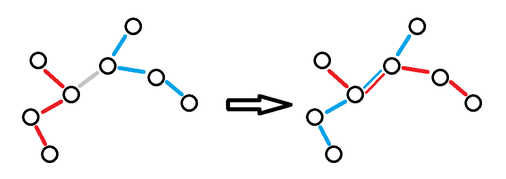
\includegraphics[width=0.5\textwidth]{p1.png} %中括号中的参数是设置图片充满文档的大小,你也可以使用小数来缩小图片的尺寸。
    \label{p1} %这是添加标签,方便在文章中引用图片。
\end{figure}%figure环境
更进一步的,我们可以得到下面这个结论:
\begin{theorem}
  对于一个树,如果它有$2k$个叶子,那么它就能被$k$条路径完全覆盖。
\end{theorem}

结论的正确性也非常显然。即如果有一条边没有被覆盖,可以通过调整两条路径得到。
\begin{figure}[h]
  \centering
  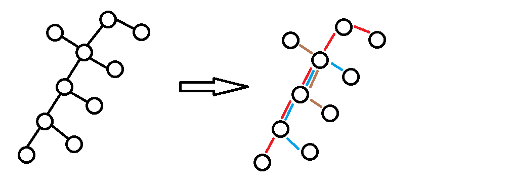
\includegraphics[width=0.5\textwidth]{p2.png}
  \label{p2}
\end{figure}

于是询问$(x,y)$可以理解为:选择$2y$个叶子,使得连通块包含$x$并且边权和最大。

我们可以考虑以$x$为根,现在的问题是如何选择叶子。

显而易见的是,如果一个节点$x$的子树中有一个叶子$u$被选择了,那么$x$所在长链包含的叶子一定也被选择了。

于是对于每一个叶子的贡献,我们单独考虑它们的贡献,贡献为它到它长链顶的距离,也就是说我们考虑一次加入长链。

于是我们按照贡献排序,依次选择即可。

但是每次都重新以$x$为根复杂度太高。我们考虑经过$x$的最长路径一定经过直径的其中一端,于是我们以直径两端分别为根做两边。

现在问题是如果$x$不被我们选择的前$2y-1$大的叶子包含怎么办?

有两种情况:一种是将贡献最小的长链去掉加入$x$所在长链,一种是找到离$x$最近的长链将下半部分替换成$x$所在长链。用倍增查找即可。

复杂度$O((n+q)\log n)$

\newpage

\end{document} 